% !TeX program = xelatex
\documentclass[border=4pt]{standalone}
\usepackage[UTF8,fontset=fandol]{ctex}
\usepackage{amsmath,amssymb,tikz,circuitikz}
\usetikzlibrary{arrows.meta,positioning,calc,fit}
\begin{document}
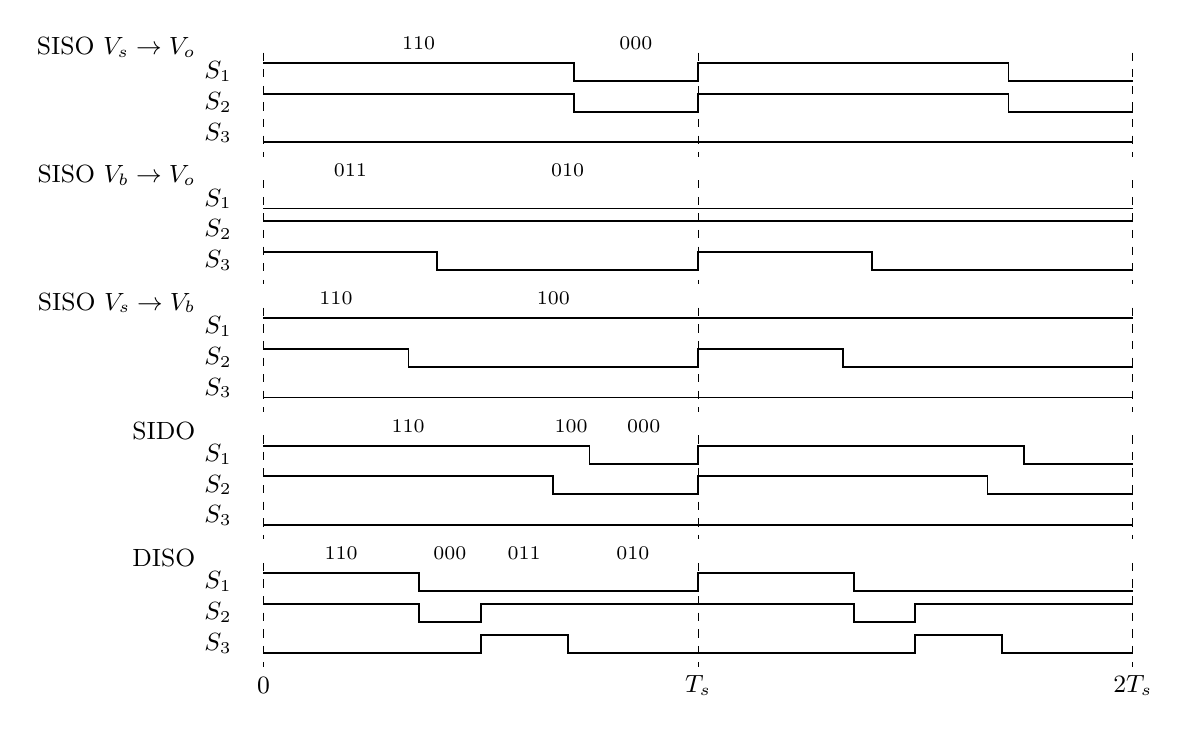
\begin{tikzpicture}[x=.92cm,y=.6cm,every node/.style={font=\small},line width=.65pt]
\node[anchor=east] at (-.5,0.7) {SISO $V_s\to V_o$};
\node[anchor=east] at (0,0.2) {$S_1$};
\draw (0.3,0.38) -- (4.584,0.38) -- (4.584,0) -- (6.3,0) -- (6.3,0.38) -- (10.584,0.38) -- (10.584,0) -- (12.3,0);
\node[anchor=east] at (0,-0.45) {$S_2$};
\draw (0.3,-0.27) -- (4.584,-0.27) -- (4.584,-0.65) -- (6.3,-0.65) -- (6.3,-0.27) -- (10.584,-0.27) -- (10.584,-0.65) -- (12.3,-0.65);
\node[anchor=east] at (0,-1.1) {$S_3$};
\draw (0.3,-1.3) -- (4.584,-1.3) -- (4.584,-1.3) -- (6.3,-1.3) -- (6.3,-1.3) -- (10.584,-1.3) -- (10.584,-1.3) -- (12.3,-1.3);
\draw[dashed,thin] (0.3,0.6)--(0.3,-1.6);
\draw[dashed,thin] (6.3,0.6)--(6.3,-1.6);
\draw[dashed,thin] (12.3,0.6)--(12.3,-1.6);
\node at (2.442,0.8) {\scriptsize 110};
\node at (5.442,0.8) {\scriptsize 000};
\node[anchor=east] at (-.5,-2) {SISO $V_b\to V_o$};
\node[anchor=east] at (0,-2.5) {$S_1$};
\draw (0.3,-2.7) -- (2.7,-2.7) -- (2.7,-2.7) -- (6.3,-2.7) -- (6.3,-2.7) -- (8.7,-2.7) -- (8.7,-2.7) -- (12.3,-2.7);
\node[anchor=east] at (0,-3.15) {$S_2$};
\draw (0.3,-2.97) -- (2.7,-2.97) -- (2.7,-2.97) -- (6.3,-2.97) -- (6.3,-2.97) -- (8.7,-2.97) -- (8.7,-2.97) -- (12.3,-2.97);
\node[anchor=east] at (0,-3.8) {$S_3$};
\draw (0.3,-3.62) -- (2.7,-3.62) -- (2.7,-4) -- (6.3,-4) -- (6.3,-3.62) -- (8.7,-3.62) -- (8.7,-4) -- (12.3,-4);
\draw[dashed,thin] (0.3,-2.1)--(0.3,-4.3);
\draw[dashed,thin] (6.3,-2.1)--(6.3,-4.3);
\draw[dashed,thin] (12.3,-2.1)--(12.3,-4.3);
\node at (1.5,-1.9) {\scriptsize 011};
\node at (4.5,-1.9) {\scriptsize 010};
\node[anchor=east] at (-.5,-4.7) {SISO $V_s\to V_b$};
\node[anchor=east] at (0,-5.2) {$S_1$};
\draw (0.3,-5.02) -- (2.304,-5.02) -- (2.304,-5.02) -- (6.3,-5.02) -- (6.3,-5.02) -- (8.304,-5.02) -- (8.304,-5.02) -- (12.3,-5.02);
\node[anchor=east] at (0,-5.85) {$S_2$};
\draw (0.3,-5.67) -- (2.304,-5.67) -- (2.304,-6.05) -- (6.3,-6.05) -- (6.3,-5.67) -- (8.304,-5.67) -- (8.304,-6.05) -- (12.3,-6.05);
\node[anchor=east] at (0,-6.5) {$S_3$};
\draw (0.3,-6.7) -- (2.304,-6.7) -- (2.304,-6.7) -- (6.3,-6.7) -- (6.3,-6.7) -- (8.304,-6.7) -- (8.304,-6.7) -- (12.3,-6.7);
\draw[dashed,thin] (0.3,-4.8)--(0.3,-7);
\draw[dashed,thin] (6.3,-4.8)--(6.3,-7);
\draw[dashed,thin] (12.3,-4.8)--(12.3,-7);
\node at (1.302,-4.6) {\scriptsize 110};
\node at (4.302,-4.6) {\scriptsize 100};
\node[anchor=east] at (-.5,-7.4) {SIDO};
\node[anchor=east] at (0,-7.9) {$S_1$};
\draw (0.3,-7.72) -- (4.296,-7.72) -- (4.296,-7.72) -- (4.8,-7.72) -- (4.8,-8.1) -- (6.3,-8.1) -- (6.3,-7.72) -- (10.296,-7.72) -- (10.296,-7.72) -- (10.8,-7.72) -- (10.8,-8.1) -- (12.3,-8.1);
\node[anchor=east] at (0,-8.55) {$S_2$};
\draw (0.3,-8.37) -- (4.296,-8.37) -- (4.296,-8.75) -- (4.8,-8.75) -- (4.8,-8.75) -- (6.3,-8.75) -- (6.3,-8.37) -- (10.296,-8.37) -- (10.296,-8.75) -- (10.8,-8.75) -- (10.8,-8.75) -- (12.3,-8.75);
\node[anchor=east] at (0,-9.2) {$S_3$};
\draw (0.3,-9.4) -- (4.296,-9.4) -- (4.296,-9.4) -- (4.8,-9.4) -- (4.8,-9.4) -- (6.3,-9.4) -- (6.3,-9.4) -- (10.296,-9.4) -- (10.296,-9.4) -- (10.8,-9.4) -- (10.8,-9.4) -- (12.3,-9.4);
\draw[dashed,thin] (0.3,-7.5)--(0.3,-9.7);
\draw[dashed,thin] (6.3,-7.5)--(6.3,-9.7);
\draw[dashed,thin] (12.3,-7.5)--(12.3,-9.7);
\node at (2.298,-7.3) {\scriptsize 110};
\node at (4.548,-7.3) {\scriptsize 100};
\node at (5.55,-7.3) {\scriptsize 000};
\node[anchor=east] at (-.5,-10.1) {DISO};
\node[anchor=east] at (0,-10.6) {$S_1$};
\draw (0.3,-10.42) -- (2.448,-10.42) -- (2.448,-10.8) -- (3.3,-10.8) -- (3.3,-10.8) -- (4.5,-10.8) -- (4.5,-10.8) -- (6.3,-10.8) -- (6.3,-10.42) -- (8.448,-10.42) -- (8.448,-10.8) -- (9.3,-10.8) -- (9.3,-10.8) -- (10.5,-10.8) -- (10.5,-10.8) -- (12.3,-10.8);
\node[anchor=east] at (0,-11.25) {$S_2$};
\draw (0.3,-11.07) -- (2.448,-11.07) -- (2.448,-11.45) -- (3.3,-11.45) -- (3.3,-11.07) -- (4.5,-11.07) -- (4.5,-11.07) -- (6.3,-11.07) -- (6.3,-11.07) -- (8.448,-11.07) -- (8.448,-11.45) -- (9.3,-11.45) -- (9.3,-11.07) -- (10.5,-11.07) -- (10.5,-11.07) -- (12.3,-11.07);
\node[anchor=east] at (0,-11.9) {$S_3$};
\draw (0.3,-12.1) -- (2.448,-12.1) -- (2.448,-12.1) -- (3.3,-12.1) -- (3.3,-11.72) -- (4.5,-11.72) -- (4.5,-12.1) -- (6.3,-12.1) -- (6.3,-12.1) -- (8.448,-12.1) -- (8.448,-12.1) -- (9.3,-12.1) -- (9.3,-11.72) -- (10.5,-11.72) -- (10.5,-12.1) -- (12.3,-12.1);
\draw[dashed,thin] (0.3,-10.2)--(0.3,-12.4);
\draw[dashed,thin] (6.3,-10.2)--(6.3,-12.4);
\draw[dashed,thin] (12.3,-10.2)--(12.3,-12.4);
\node at (1.374,-10) {\scriptsize 110};
\node at (2.874,-10) {\scriptsize 000};
\node at (3.9,-10) {\scriptsize 011};
\node at (5.4,-10) {\scriptsize 010};
\node at (.3,-12.8) {$0$};\node at (6.3,-12.8) {$T_s$};\node at (12.3,-12.8) {$2T_s$};\end{tikzpicture}
\end{document}
